\documentclass{article}

\usepackage{graphicx}
\usepackage{tikz}
\usepackage{tikzsymbols}
\usetikzlibrary{calc,patterns,shapes.geometric}
\pagestyle{empty}
\usepackage[margin=0pt]{geometry}
\geometry{papersize={14in,12in}}

\def\centerarc[#1](#2)(#3:#4:#5){\draw[#1] ($(#2)+({#5*cos(#3)},{#5*sin(#3)})$) arc (#3:#4:#5);}

\begin{document}
	\begin{figure}
		\centering
		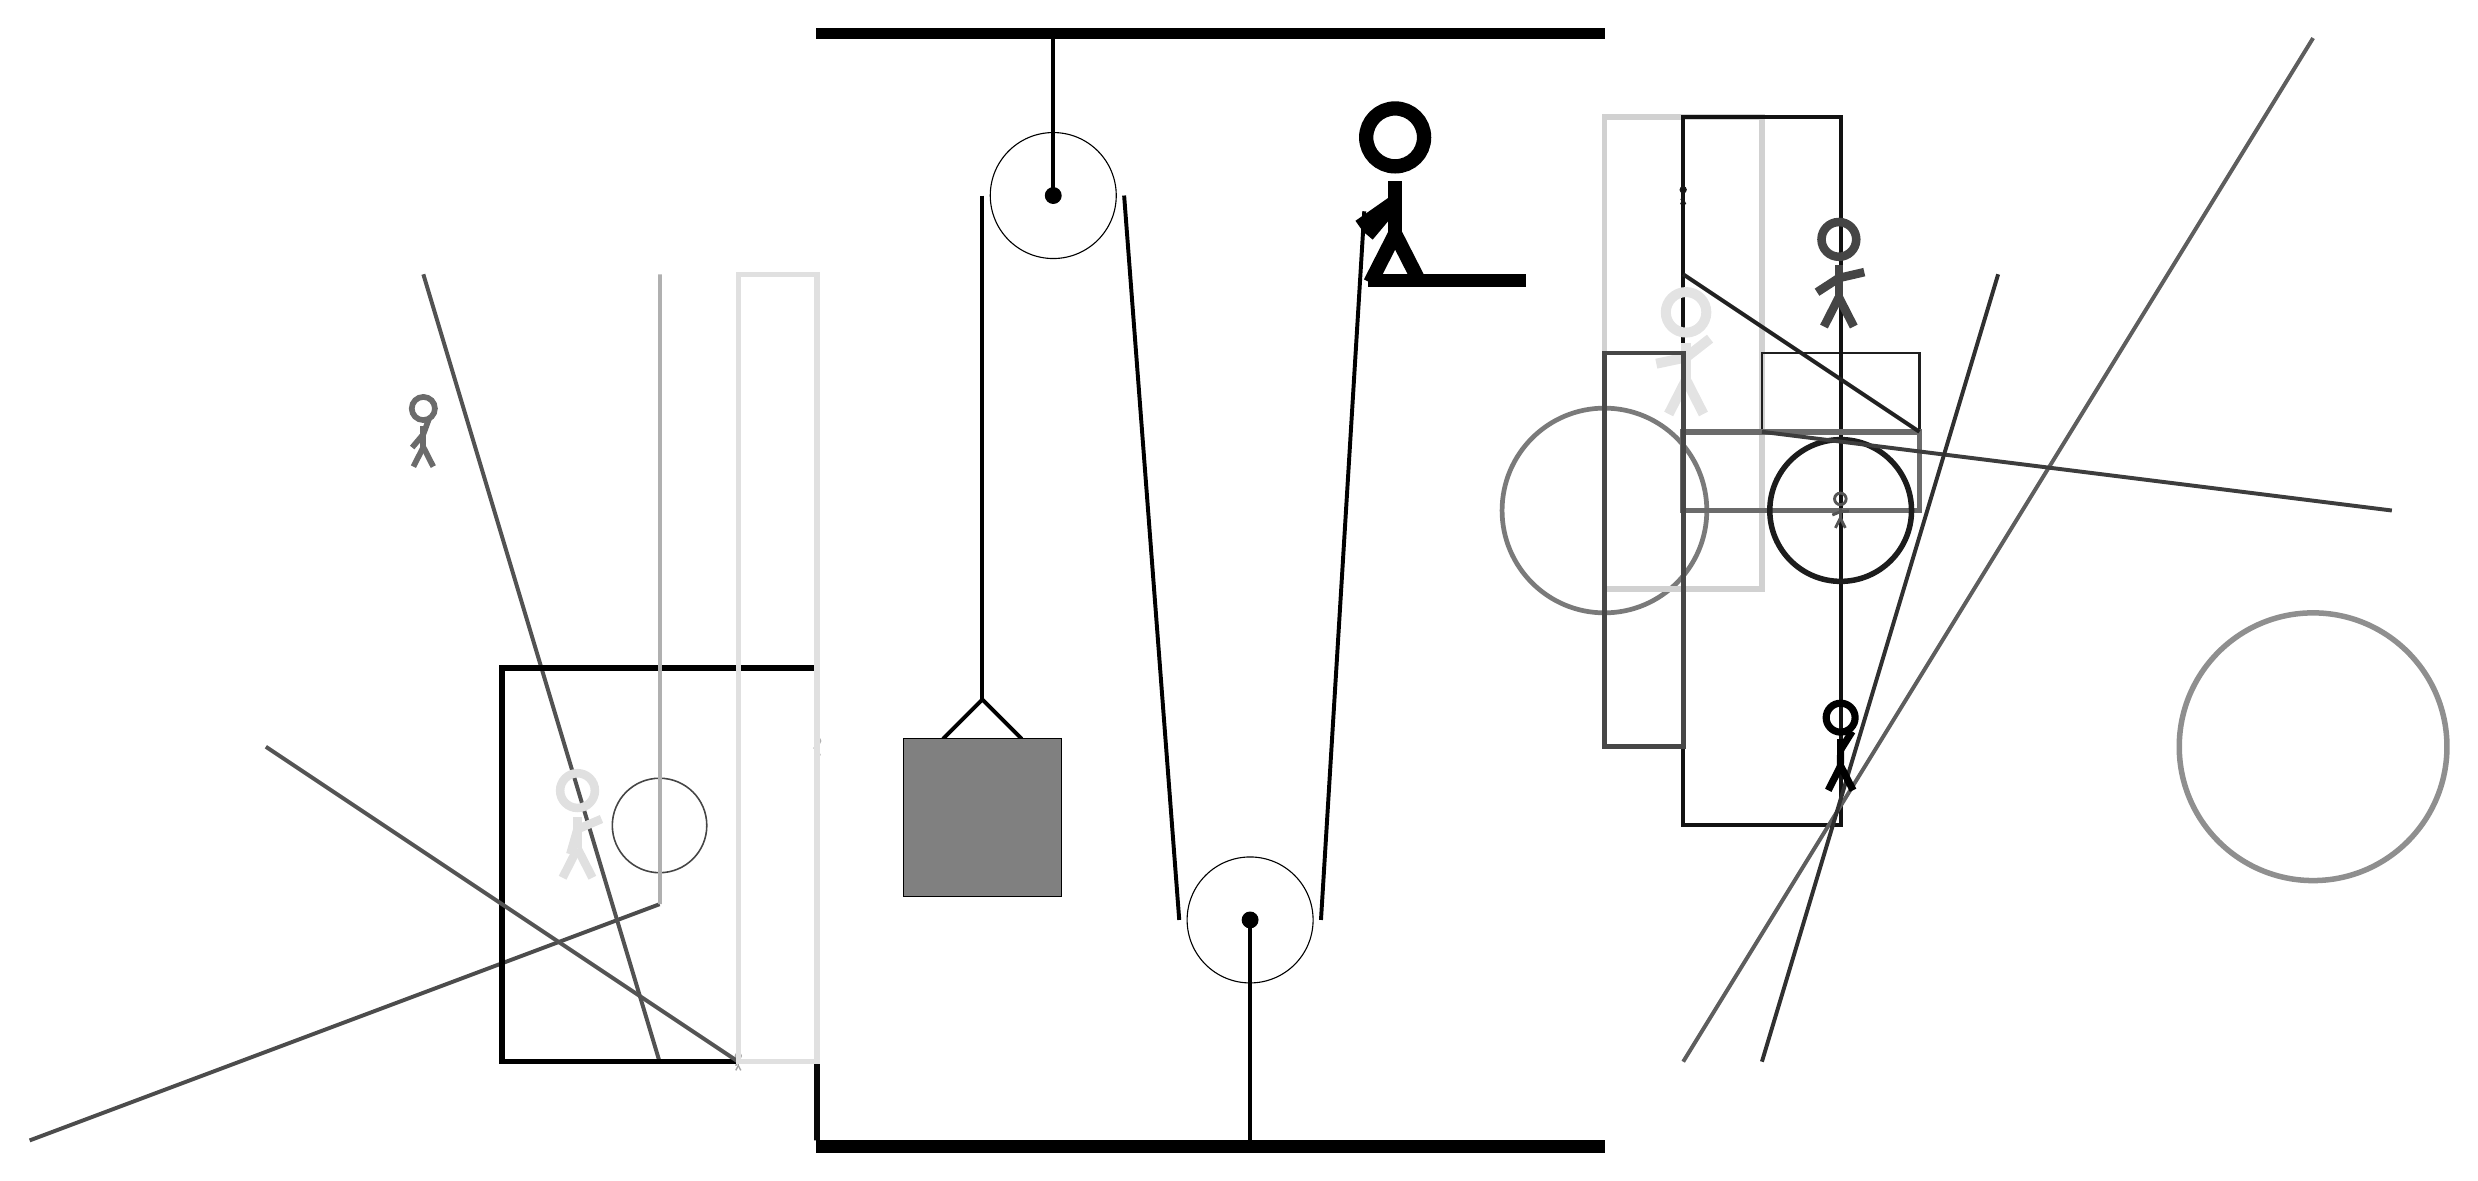
\begin{tikzpicture}
			%%%%% START %%%%%
			
			\draw[fill=black] (-2, 14) rectangle (8, 14.125);
			
			\draw (3.5, 2.8) circle (0.8);
			\draw[fill=black] (3.5, 2.8) circle (0.1);
			\draw[line width=0.5mm] (3.5, 2.8) -- (3.5, 0);
			
			\draw (1, 12) circle (0.8);
			\draw[fill=black] (1, 12) circle (0.1);
			\draw[line width=0.5mm] (1, 14) -- (1, 12);
			
			\draw[line width=0.5mm](-0.4, 5.1) --  (0.1, 5.6) -- (0.6, 5.1);
			\draw[fill=black!50] (-0.9, 5.1) rectangle (1.1, 3.1);
			
			\draw[line width=0.5mm](0.1, 12) -- (0.1, 5.6);
			\centerarc[line width=0.5mm](1, 12)(180:0:0.9)
			\draw[line width=0.5mm](1.9, 12) -- (2.6, 2.8);
			\centerarc[line width=0.5mm](3.5, 2.8)(180:360:0.9)
			\draw[line width=0.5mm](4.4, 2.8) -- (4.95, 11.8);
			
			\draw [line width=0.2mm, color=black!73](-4, 4) circle (0.6);
			
			\draw [line width=0.6mm, color=black!52](8, 8) circle (1.3);
			\draw[line width=0.5mm, color=black!86](9, 9) -- (9, 6);
			\draw[line width=0.7mm, color=black!18] (8, 13) rectangle (10, 7);
			\node[line width=0.3mm, color=black!36] at (-3, 1) {\Strichmaxerl[1][50][61]};
			\node[line width=0.5mm, color=black!58] at (-7, 9) {\Strichmaxerl[4][50][70]};
			\draw[line width=0.5mm, color=black!70](-4, 3) -- (-12, 0);
			\draw[line width=0.3mm, color=black!88] (10, 9) rectangle (12, 10);
			\draw[line width=0.5mm, color=black!93] (9, 4) rectangle (11, 13);
			
			\draw[line width=0.7mm, color=black!58] (9, 8) rectangle (12, 9);
			\draw[line width=0.5mm, color=black!63](9, 1) -- (17, 14);
			
			\draw[line width=0.5mm, color=black!68](-4, 1) -- (-7, 11);
			\node[line width=0.3mm, color=black!67] at (11, 8) {\Strichmaxerl[2][22][5]};
			
			\node[line width=0.2mm, color=black!11] at (9, 10) {\Strichmaxerl[7][12][38]};
			\draw [line width=0.7mm, color=black!89](11, 8) circle (0.9);
			\draw[line width=0.5mm, color=black!76](10, 9) -- (18, 8);
			
			\node[line width=0.4mm, color=black!73] at (11, 11) {\Strichmaxerl[6][33][13]};
			
			\draw[line width=0.5mm, color=black!87](12, 9) -- (9, 11);
			\node[line width=0.2mm, color=black!31] at (-2, 5) {\Strichmaxerl[1][11][78]};
			\draw[line width=0.5mm, color=black!81](13, 11) -- (10, 1);
			\node[line width=0.7mm, color=black!91] at (9, 12) {\Strichmaxerl[1][60][84]};
			
			\draw [line width=0.7mm, color=black!44](17, 5) circle (1.7);
			\draw[line width=0.7mm, color=black!97] (-2, 0) rectangle (-2, 11);
			\node[line width=0.4mm, color=black!100] at (11, 5) {\Strichmaxerl[5][89][58]};
			\draw[line width=0.7mm, color=black!100] (-2, 1) rectangle (-6, 6);
			
			\draw[line width=0.5mm, color=black!31] (-4, 3) rectangle (-4, 11);
			\draw[line width=0.5mm, color=black!67](-3, 1) -- (-9, 5);
			\node[line width=0.7mm, color=black!12] at (-5, 4) {\Strichmaxerl[6][74][23]};
			
			\draw[line width=0.6mm, color=black!72] (8, 5) rectangle (9, 10);
			
			\draw[line width=0.7mm, color=black!12] (-3, 11) rectangle (-2, 1);
			
			\node at (5.3, 12) {\Strichmaxerl[10][35][-130]};
			\draw[fill=black] (5, 11) rectangle (7, 10.85);
			
			\draw[fill=black] (-2, 0) rectangle (8, -0.15);
			
			%%%%% END %%%%%
		\end{tikzpicture}
	\end{figure}	
\end{document}